\section{Validation}
To validate the first version of the Scalability Testing Framework, we developed two distributed applications. The first one, a distributed matrix multiplication, is a simple application that can have two different scalability sizes with a small change in the implementation. Thus, we used it to compare the scalability of two similar applications, and to validate if our framework was capable of showing the difference between them.

The second one is a choreography to be our test bed of the framework for this initial validation, and future researches. It offers a service that buys a product list from a set of supermarkets with the best price.

\subsection{Distributed Matrix Multiplication Validation}

The Distributed Matrix Multiplication service is a simple distributed application that multiplies two matrices. There is a central node that receives the request and coordinates the multiplication. It requests to other nodes to multiply parts of the matrices.

We used a simple matrix multiplication algorithm that is presented at Code~\ref{MMAlgorithm}. The first \emph{for} iterates over the lines of matrix A, and the second one iterates over the columns of matrix B. Thus, for each line $i$ of matrix A the algorithm multiplies all columns of matrix B to calculate each line $i$ of matrix C. This algorithm involves $\theta(n^3)$ operations, since it has three \emph{for}s of $n$ interactions each one.
\lstset{caption={Matrix Multiplication Algorithm},label=MMAlgorithm}
\begin{lstlisting}
double[][] multiplyMatrix(double[][] A, double[][] B, int n) {
	double[][] C = new double[n][n];
	
	for(int i = 0; i<n; i++) {
		for(int j = 0; j<n; j++) {
			C[i][j] = 0.0;
			for(int k = 0; k<n; k++)
				C[i][j] = C[i][j] + A[i][k]*B[k][j];
		}
	}
	return C;
}
\end{lstlisting}

We can parallel this algorithm by requesting each node of the system to multiply just a range of the matrix B columns. Thus, each node will return a range of the matrix C columns as we can see in Figure \ref{matrices}.

\begin{figure}[htbp]
\begin{center}
	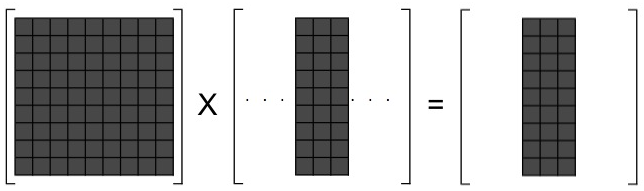
\includegraphics[scale=0.5]{images/matrices}
\caption{Distributed Matrix Multiplication of a Node}
\label{matrices}
\end{center}
\end{figure}

The resulted algorithm of each node is presented in the Code~\ref{DMMAlgorithm}. Only the columns from \emph{min} to \emph{max} of matrix B are used to calculate the same columns of matrix C. If each node calculates its part in parallel the algorithm will be executed $Q$ times faster, which Q is the number of nodes. If they are not executed in parallel, the time will be the same of the first algorithm presented.
\clearpage

\lstset{caption={Distributed Matrix Multiplication Algorithm},label=DMMAlgorithm}
\begin{lstlisting}
double[][] multiplyMatrix(double[][] A, double[][] B, int min, int max, int n) {
	double[][] C = new double[n][n];
	
	for(int i = 0; i<n; i++) {
		for(int j = min; j<max; j++) {
			C[i][j] = 0.0;
			for(int k = 0; k<n; k++)
				C[i][j] = C[i][j] + A[i][k]*B[k][j];
		}
	}
	return C;
}
\end{lstlisting}

A distributed application was developed with Java RMI for the communication between the service that coordinates the multiplication, and the services that multiply part of the matrices. Java RMI (Remote Method Invocation) allows the communication between objects of different JVMs~[\citet{JavaRMI}]. One object can manipulate another remote object in the same way it manipulates a local one. The JVM abstracts the lower layers of communication.

We used JAX-WS\footnote{http://jax-ws.java.net/}, a Java API for XML Web Services, to provide this service as a web service.  This web service receives a request with the number of nodes that it must use, and the size of the two matrices to multiply. It coordinates the multiplication communicating with the Java RMI servers that multiply parts of the matrices. Figure~\ref{dmm} presents the structure of the application. They were deployed in the Amazon EC2\footnote{http://aws.amazon.com/ec2/}, the Amazon cloud environment.

\begin{figure}[htbp]
\begin{center}
	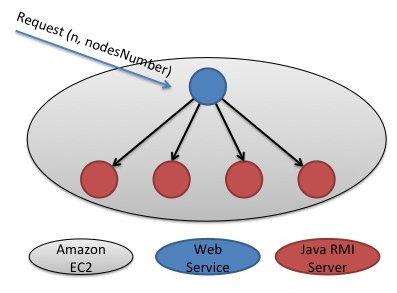
\includegraphics[scale=0.6]{images/dmm}
\caption{Distributed Matrix Multiplication Structure}
\label{dmm}
\end{center}
\end{figure}

Two coordinators were implemented with two approaches to validate our framework. In the first one, we supposed that the developer made a mistake by implementing the interation sequentially. It requests the multiplication for each node after the calculation of the last one. In the second implementation, the requests are made in parallel. Thus, all nodes multiply parts of the matrices in the same time.

\subsubsection{Scalability Testing}
To verify the scalability of the distributed matrix multiplication service, we need to follow the steps described in the begging of Section~\ref{framework}. First, we needed to define the variables that define the scalability function (Step 1):
\begin{description}
\item[Problem complexity variable: ] Matrix size, $n$.
\item[Performance variable: ]  Response time, $M$.
\item[Architecture variable: ] Number of nodes, $Q$.
\end{description}

Then, we needed to define how the functions that use these variables will be (Step 2):
\begin{description}
\item[Complexity size of the problem: ] $n^3$
\item[Performance metric: ]  $M$ 
\item[Architecture capability: ] $Q$
\end{description}

Thus, the scalability function is $\frac{n^3M}{Q}$ and it is expected to be constant. Since we chose to increase the complexity size of the problem and the architecture capability with the same proportion, the response time of each execution should be constant. 

After that, we chose the initial values of them(Step 3). For this experiment, the initial value of $n$ and $Q$ were $400$ and $1$, respectively. 

The steps 4 to 6 were done using the Scalability Testing Framework. Code \ref{MMP} shows a scalability test for the service that implements the algorithm in parallel. The first decision made was the number of steps we wanted to make and how the variables would increase (Line 1). The number of steps chosen was 8  because of the limitation of nodes that Amazon EC2 provides. For this reason too, we chose to increase the variables linearly to execute more steps. If we had chosen to increase exponentially, for instance, the framework could only execute 4 steps, because the number of nodes in each step would be: 1, 2, 4, and 8.

\lstset{caption={Matrix Multiplication in Parallel},label=MMP}
\begin{lstlisting}
@ScalabilityTest(steps = 8, scalabilityFunction = LinearIncrease.class)
public ArrayList<Long> multOfTwoMatrices(@Scale int numberOfNodes) 
		throws Exception {
	WSClient wsClient = new WSClient(
			AMAZON_WS_URL + "multiplyMatrices?wsdl");
	int n = getNBasedOnNumberOfNodes(numberOfNodes);
	Item item = generateItem(n, numberOfNodes);
	ArrayList<Long> results = new ArrayList<Long>();
	for (int i = 0; i < REPETITIONS; i++) {
		Long start = System.currentTimeMillis();
		wsClient.request("multiplyMatrices", item);
		Long end = System.currentTimeMillis();
		results.add(end - start);			
	}
	return results;
}
\end{lstlisting}

To increase the complexity size of the problem linearly, we needed to choose arbitrarily the $n_i$ based on the number of nodes. Table \ref{table1} shows the chosen $n$s for each step. As we can see, the architecture capability and the complexity size of the problem stay with the same proportion. Therefore, we only pass the number of nodes as an argument because the value of $n$ is based on it, using the function \emph{getNBasedOnNumberOfNodes} (Line 6).

\begin{table}[htdp]
\caption{Relation between $Q$ and $n$}
\begin{center}
\begin{tabular}{|c|c|c|}
\hline
$Q$ 	& $n$ 	& $n^3/Q$ \\ \hline
$1$	& $400$	& $64 \times 10^6$ \\ \hline
$2$	& $504$	& $\sim64 \times 10^6$ \\ \hline
$3$	& $577$	& $\sim64 \times 10^6$ \\ \hline
$4$	& $635$	& $\sim64 \times 10^6$ \\ \hline
$5$	& $684$	& $\sim64 \times 10^6$ \\ \hline
$6$	& $727$	& $\sim64 \times 10^6$ \\ \hline
$7$	& $765$	& $\sim64 \times 10^6$ \\ \hline
$8$	& $800$	& $64 \times 10^6$ \\ \hline

\end{tabular}
\end{center}
\label{table1}
\end{table}%

At line 4, we create a client dynamically, using the a component of the Rehearsal Framework, to communicate with the web service. The message that is sent is created at line 7. 

More than one request is made for each step to avoid values very different from the usual. The number of requests made are defined in the constant \emph{REPETITIONS}, which is 30, in this case. For each step, a list of response times is returned. The framework is responsible for calculating the mean and the standard deviation of them.

The framework executes this method 8 times, increasing the parameter \emph{numberOfNodes}. For each execution, it collects the results and calculates the mean and the standard deviation. The result is passed as a ScalabilityReport object. In the code \ref{call} , we request the execution of two scalability tests, one for the service that executes the algorithm in parallel (Line 1), and another for the service that executes the algorithm sequentially (Line 2).

\lstset{caption={Scalability Tests Call and Plot Results in a Graph Code},label=call}
\begin{lstlisting}
ScalabilityReport report1 = ScalabilityTesting.run(tests, "multOfTwoMatrices", 1);
ScalabilityReport report2 = ScalabilityTesting.run(tests, "multOfTwoMatricesSeq", 1);

ScalabilityReportChart chart = new ScalabilityReportChart();
List<ScalabilityReport> reports = new ArrayList<ScalabilityReport>();
reports.add(report1);
reports.add(report2);
chart.createChart(reports, "Execution time (ms)");
\end{lstlisting} 

The class that plots the scalability test graph is the \emph{ScalabilityReportChart} (Line 4). It receives a list of reports and plot them in a graph. Thus, at line 5 to 7, we create a list of \emph{ScalabilityReport}s to generate the graph (Line 8).

The graph created by the framework is presented in Figure~\ref{dmmGraph}. The blue line is the result for the service that implements the algorithm sequentially. It has a bad scalability, comparing to the red line which is the parallel approach. It is similar to the bad scalability graph described in Image~\ref{fig:badscalability} while the red line is similar to the good scalability graph described in Image~\ref{fig:goodscalability}.

\begin{figure}[htbp]
\begin{center}
	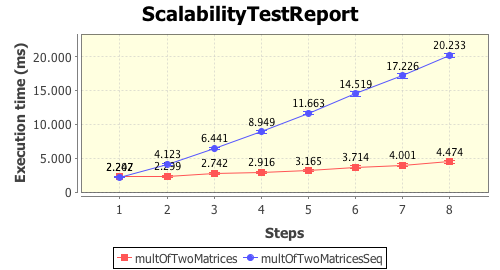
\includegraphics[scale=0.8]{images/twoTestsReportLinear8}
\caption{Scalability Testing Results Graph}
\label{dmmGraph}
\end{center}
\end{figure}

However, if we only see the result of the service with the parallel approach in Figure~\ref{dmmParallelGraph}, we can also say that it has a bad scalability because it increases as well. Nevertheless, we concluded in section~\ref{scalabilityTesting} that scalability is something relative. It is highly dependent on the chosen variables. 

It is easier to verify the scalability of an application when we are comparing to another implementation. With the absence of another, the definition of some bounds can assist the scalability explorer to analyze the scalability. For instance, in Figure~\ref{dmmParallelGraph}, if we define that the service response time must be less then 5 seconds, then we conclude that the service is scalable until 8 nodes with matrices os size less than 800. 

\begin{figure}[htbp]
\begin{center}
	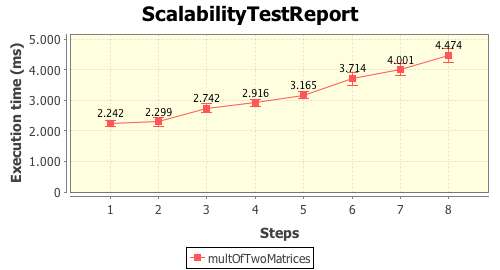
\includegraphics[scale=0.8]{images/multiplicationOfTwoMatricesReport8}
\caption{Scalability Testing Result Graph for the Parallel Approach Service}
\label{dmmParallelGraph}
\end{center}
\end{figure}



\subsection{Choreography Validation}
We developed a web service choreography to be our test bed for getting information and developing the Rehearsal Framework. Thus, we will use this choreography to collect information about how we are going to verify its scalability. In this section, we will explain how it works.

The choreography implements a service of a supermarket of the future. Based on a list of supermarkets, we are able to get the lowest price possible of a desired product list. For each product, the choreography gets the price from the supermarket that offers the lowest. Therefore, we will purchase a list of products with the lowest possible price from a list of supermarkets.

\subsubsection{Participants of the choreography}
\label{participantschoreography}

The choreography has five participants. Their roles and API are described bellow:
\begin{description}
\item[SMRegistry] The SMRegistry service stores a list of services that implements the supermarket role. Its methods are presented on Table \ref{smregistryapi}.
	\begin{table}[htdp]
	\caption{SMRegistry API}
	\begin{center}
	\begin{tabular}{|c|c|c|m{4cm}|}
		\hline
		Method & Input & Output & Description \\ \hline
		addSupermarket & endpoint : String & confirmation : String & Add a new supermarket endpoint to the supermarket list \\ \hline
		getList & & supermarkets: List<String> & Return a list of supermarket endpoints \\ \hline
	\end{tabular}
	\end{center}
	\label{smregistryapi}
	\end{table}%

\item[SupermarketRole] The choreography can have multiple supermarkets, each supermarket must implement the Supermarket Role API, presented on Table \ref{smroleapi}. It must return the price of a product, and purchase a list of products.
	\begin{table}[htdp]
	\caption{Supermarket Role API}
	\begin{center}
	\begin{tabular}{|c|m{3.5cm}|m{3.5cm}|m{4cm}|}
		\hline
		Method				& Input						& Output 					& Description \\ \hline
		searchForProduct 		& name: String					& name: String, price: Double 	& Get the product price of this supermarket \\ \hline
		registerSupermarket		& endpoint: String				& confirmation: String		& Register the Supermarket endpoint in the RegistrySM service \\ \hline
		purchase				& id: String, personalDataType: data & confirmation: String		& Make the purchase with the order ID and the user address \\ \hline
	\end{tabular}
	\end{center}
	\label{smroleapi}
	\end{table}%
	
\item[Customer] The Customer service is the interface of the choreography. The user can communicates with the other service separately, however the complete functionalities of the choreography are accessible by this service. Its implementation is an orchestration that communicates with the SMRegistry service to get the list of Supermarket services registered. It communicates with all of them to get the minimum price possible of the product list. After returning the order, the user can communicates with the Customer to request a purchase and the delivery informations. Its API is presented on Table \ref{customerapi}.
	\begin{table}[htdp]
	\caption{Customer API}
	\begin{center}
	\begin{tabular}{|c|m{3.5cm}|m{3.5cm}|m{4cm}|}
		\hline
		Method				& Input					& Output 					& Description \\ \hline
		getPriceOfProductList	& products: List<String> & order: Order & Return the minimum price of a product list and the id of the order\\ \hline
		purchase 				& id: String, account: accountType & shipper: String & Make the purchase of the products requested with the operation above \\ \hline
		getDeliveryData 		& shipper: String, orderID: String & delivery: String & Get information about the delivery of an order \\ \hline
		
	\end{tabular}
	\end{center}
	\label{customerapi}
	\end{table}%

\item[Shipper] The Shipper service is responsible for storing information about the delivery of products to an address. The shipper receives information about an order from a Supermarket service and sends delivery information of an order to the Custumer Service. Table \ref{shipperapi} shows its API.

	\begin{table}[htdp]
	\caption{Shipper API}
	\begin{center}
		\begin{tabular}{|c|c|c|m{4cm}|}
		\hline
		Method			& Input					& Output 					& Description \\ \hline
		setDelivery		& id: String, zipcode: String	& confirmation: String		& Receives the zipcode of an order \\ \hline
		getDataAndTime	& id: String				& time: String				& Returns the time that the order will be delivered \\ \hline
	\end{tabular}
	\end{center}
	\label{shipperapi}
	\end{table}%
	\end{description}
	
\subsubsection{The workflow}
The choreography has three operations as described in the participant Customer of Subsection \ref{participantschoreography}. Before purchasing a list of products, the user must send this list to the Customer to book them and verify the price. After that, the user can purchase them providing the \emph{id} of the order. Finally, its possible to verify the delivery status to know when the product will arrive. Another message flow that does not happen with these operations is the registering of a Supermarket service in the RegistrySM service. Figure \ref{futuremartConversation} describes a global view of the conversation between the services using BPMN2\footnote{http://www.bpmn.org}.

\begin{figure}[htbp]
\begin{center}
	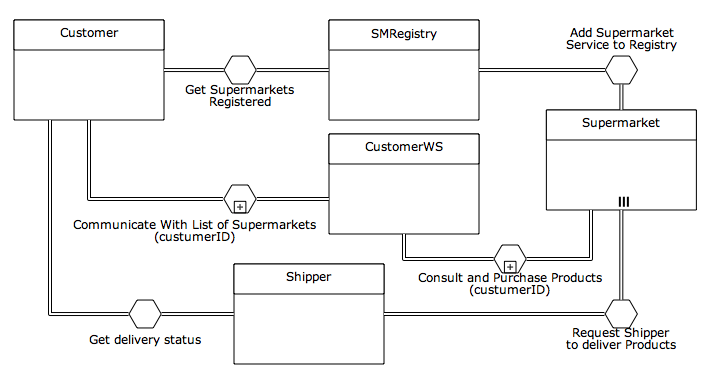
\includegraphics[width=\textwidth]{images/futuremartConversation}
\caption{Global conversation between the services of the Futuremart Choreography}
\label{futuremartConversation}
\end{center}
\end{figure}

\paragraph{The \emph{getPriceOfProductList} workflow\\}
Figure \ref{getPriceOfProductListworkflow} shows a BPMN Collaboration diagram of the getPriceOfProductList operation. Each lane represents a participant of the choreography. The getPriceOfProductList operation starts with the Customer participant receiving a request with a list of products. It requests a list of Supermarket services registered to the SMRegistry participant. The registry service collects, from its database, all service endpoints stored, and returns it to the Customer.

The Customer stores this list and the product list in its database. Then, it calculates the minimum price possible. The process that calculates the price requests, for each product,  the product price to all Supermarkets.  

The Supermarket lane represents all Supermarket services, the three little vertical lines inside it symbolize a multiplicity of participants. When each of them receives a request, it verifies in its database what is the price for the specific product to return to the Customer. If the price received is lower then the current lowest, it stores it with the endpoint of the Supermarket service that offers it. 

After checking out and storing all the products price with their respective supermarkets, the Customer returns the price and an id that represents this order.

\begin{figure}[htbp]
\begin{center}
	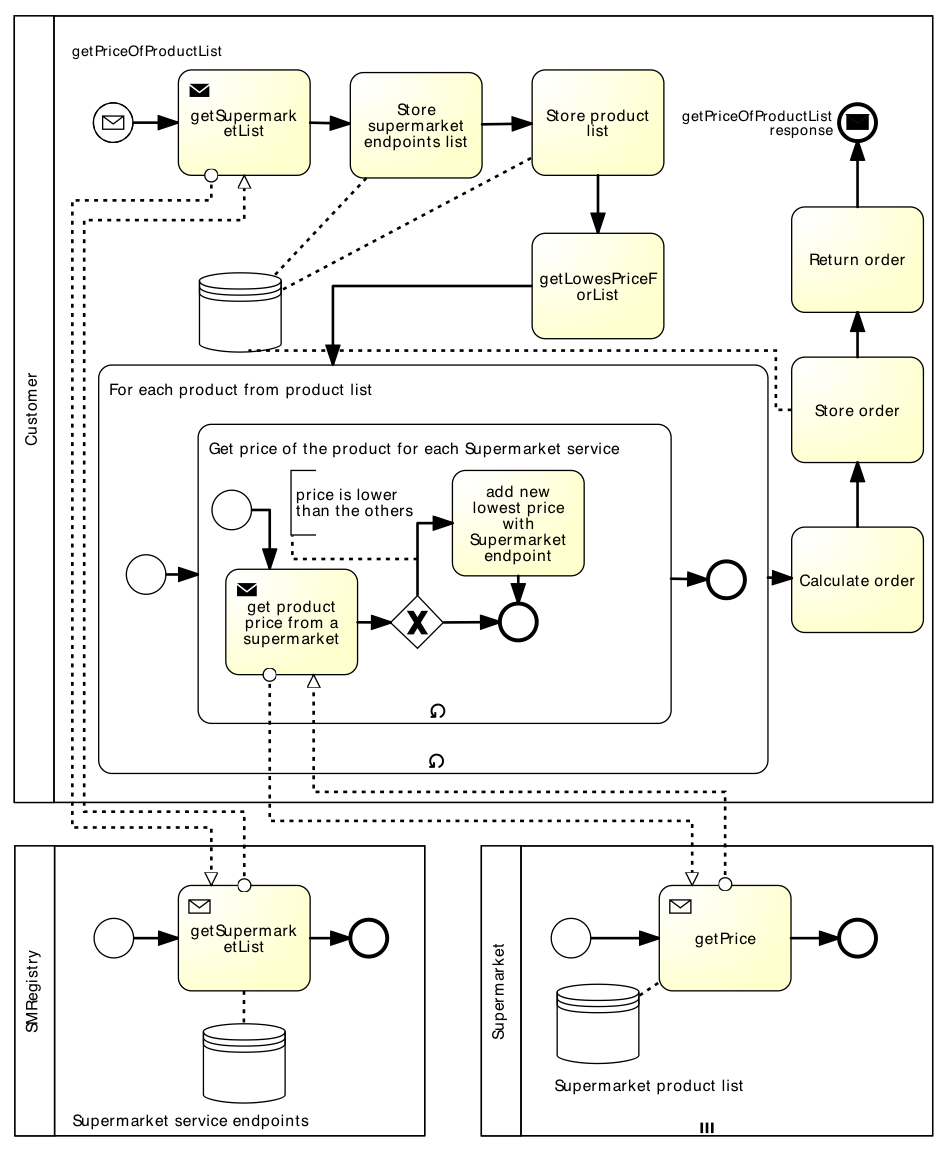
\includegraphics{images/getPriceOfProductListworkflow} 
\caption{BPMN Collaboration diagram of the choreography operation \emph{getPriceOfProductList}}
\label{getPriceOfProductListworkflow}
\end{center}
\end{figure}

\paragraph{The \emph{purchase} workflow\\}
After ordering a list of products and getting the best price for it, the user can request the purchase. The Customer service receives the request with the order ID and the address of the user. Subsequently, the service starts a loop that purchases the products related to each Supermarket service.

When a Supermarket service receives a purchase request, it sends a message to the Shipper service to deliver the products. After that, it returns a message to the Customer with the Shipper service endpoint that will deliver the products.

The Shipper service stores the delivery information in its database for future verifications. Finally, the Customer service returns to the user a confirmation with the Shipper service endpoint that will deliver the products. Figure \ref{purchaseworkflow} describes the collaboration between the services that participates in this functionality.

\begin{figure}[htbp]
\begin{center}
	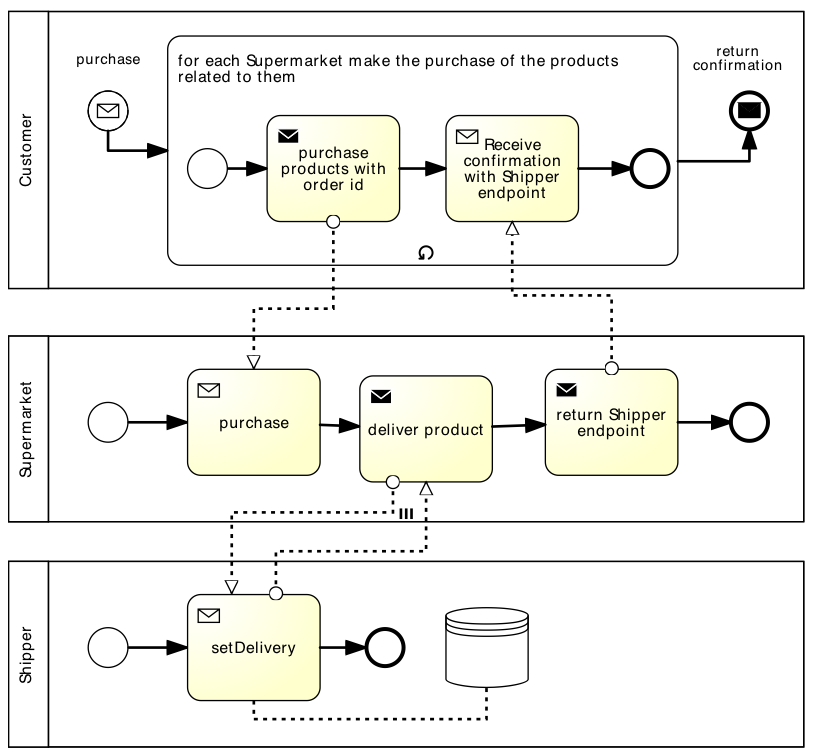
\includegraphics{images/purchaseworkflow}
\caption{BPMN Collaboration diagram of the choreography operation \emph{purchase}}
\label{purchaseworkflow}
\end{center}
\end{figure}

\paragraph{The \emph{getDeliveryData} workflow\\}
The user can also verify the delivery status of an order. The Customer service has the getDeliveryData operation that receives an order ID, and the Shipper service endpoint. It sends a message to the Shipper requesting the status of an order. The latter collects the order information  from its database and returns it. As we can see in Figure \ref{getDeliveryDataworkflow}, the Customer simply returns these data to the user.

\begin{figure}[htbp]
\begin{center}
	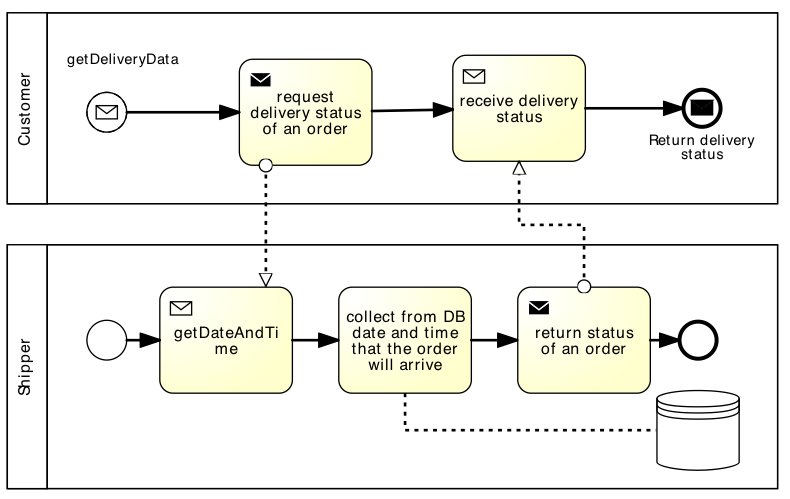
\includegraphics{images/getDeliveryDataworkflow}
\caption{BPMN Collaboration diagram of the choreography operation \emph{getDeliveryData}}
\label{getDeliveryDataworkflow}
\end{center}
\end{figure}

\paragraph{The \emph{registerSupermarket} workflow\\}
The registerSupermarket operation is not for the final user of the choreography, but for the user that administrates a Supermarket service. A service that implements the Supermarket role can register itself into the RegistrySM service, that has a list of all Supermarket services. Figure \ref{registerSupermarketworkflow} describes this registration. A Supermarket service sends a message to register itself. The registrySM service receives this request, stores the service endpoint in its database, and returns a confirmation.

\begin{figure}[htbp]
\begin{center}
	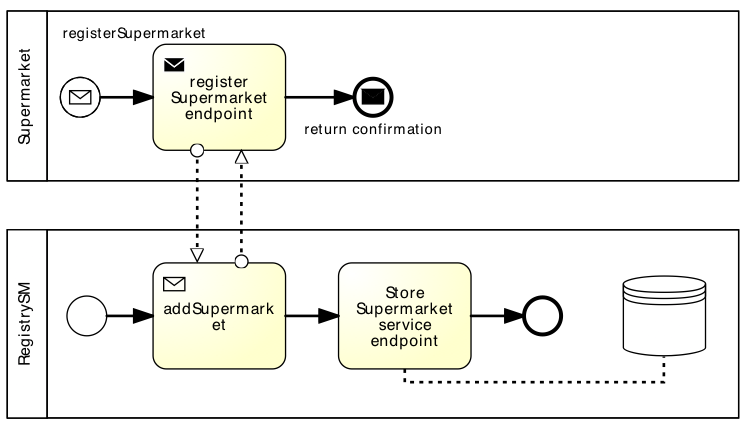
\includegraphics{images/registerSupermarketworkflow}
\caption{BPMN Collaboration diagram of the choreography operation \emph{registerSupermarket}}
\label{registerSupermarketworkflow}
\end{center}
\end{figure}

\clearpage
\subsubsection{Testing the choreography}

